\documentclass[letterpaper]{article}
% \usepackage{natbib}
\usepackage[utf8]{inputenc}
%\usepackage[margin=7cm]{geometry}
% \usepackage{listings}
% \usepackage{adjustbox}
% \usepackage{xcolor}
% \usepackage{verbatim}
% \usepackage{graphicx}%images
% \usepackage{fancyhdr}%for headers and footers
% \usepackage{adjustbox}
% \usepackage{verbatim}
% \usepackage{listings}
% \usepackage{fancyhdr}
% \usepackage{multirow}
% \usepackage{amsmath}
% \usepackage{mathtools}

% \usepackage{array}
% \usepackage{subcaption}
% \usepackage{float}
% \usepackage{csvsimple}
% \usepackage{filecontents}
% \usepackage{lscape}
% \usepackage{afterpage}
% \usepackage{hyperref}
% \usepackage{inconsolata}
% \usepackage{color}

\usepackage{mathpazo}
\usepackage{amsmath,amsfonts,amssymb,amsthm}
\usepackage{mathtools}
\usepackage{todonotes}


\usepackage{tikz}
\usetikzlibrary{arrows}

% \usepackage{draftwatermark}
% \SetWatermarkText{Draft}
% \SetWatermarkScale{2}

% Math function

\DeclarePairedDelimiter{\ceil}{\lceil}{\rceil}
\DeclarePairedDelimiter{\floor}{\lfloor}{\rfloor}
\DeclarePairedDelimiter{\tuple}{\langle}{\rangle}
\newcommand{\darrow}{\, \downarrow \!\!}
\newcommand{\uarrow}{\, \uparrow \!\!}

% Theorems styles

\theoremstyle{definition}
\newtheorem{proposition}{Proposition}[subsection]
\newtheorem{example}{Example}[subsection]

% \newenvironment{conditions}
%   {\par\vspace{\abovedisplayskip}\noindent\begin{tabular}
%   {>{$}l<{$} @{${}={}$} l}}
%   {\end{tabular}\par\vspace{\belowdisplayskip}}
%
%
%   \newenvironment{conditions_bis}
%   {\par\vspace{\abovedisplayskip}\noindent\begin{tabular}
%   {>{$}l<{$} @{${}\in{}$} l}}
%   {\end{tabular}\par\vspace{\belowdisplayskip}}
%
% \definecolor{pblue}{rgb}{0.13,0.13,1}
% \definecolor{pgreen}{rgb}{0,0.5,0}
% \definecolor{pred}{rgb}{0.9,0,0}
% \definecolor{pgrey}{rgb}{0.46,0.45,0.48}
%
% \lstset{language=Python,
%   showspaces=false,
%   numbers=left,
%   showtabs=false,
%   breaklines=true,
%   showstringspaces=false,
%   breakatwhitespace=true,
%   commentstyle=\color{pgreen},
%   keywordstyle=\color{pblue},
%   stringstyle=\color{pred},
%   basicstyle=\ttfamily,
%   moredelim=[il][\textcolor{pgrey}]{$ $},
%   moredelim=[is][\textcolor{pgrey}]{\%\%}{\%\%}
% }
%
%
%
% \hypersetup{
%     colorlinks,
%     citecolor=black,
%     filecolor=black,
%     linkcolor=black,
%     urlcolor=black
% }
%
%
% % ------ HEADERS AND FOOTERS -----------
% % \lhead{INFO-F403}
% % \rhead{Project Report - Part 1}
% %\pagestyle{fancy}
% % \rfoot{\thepage}
% %\cfoot{}
% %\lfoot{Academic Year 2017-18}
%
\newcommand{\HRule}{\rule{\linewidth}{0.2mm}} %newcommand for cover page


\begin{document}

\begin{titlepage}

\begin{center}


\textsc{\LARGE universit\'e libre de bruxelles}\\[1.0cm]
\textsc{\Large D\'epartment d'Informatique}\\[1.0cm]

% Upper part of the page. The '~' is needed because \\
% only works if a paragraph has started.

\includegraphics[width=0.3\textwidth]{images/ulblogo.jpg}~\\[1cm]

\textsc{
\large MEMO-F-403 \\
\Large  Preparatory work for the master thesis
 \\[1.0cm]}
% Title
\HRule \\[0.3cm]

{ \huge \bfseries Implementing data structures for
Partially Ordered Set \\[0.3cm] }

\HRule \\[1cm]

% Author and supervisor
\noindent
\begin{center} \large

%\emph{Author:}\\
\Large Hakim \textsc{Boulahya}\\
\end{center}
\begin{center} \large

\emph{Supervised by} \\
\Large Emmanuel \textsc{Filiot} \\

\end{center}

\\[1cm]
% Bottom of the page
{\large \today}

\end{center}
\end{titlepage}


% \title{Implementing data structures for \\ Partially Ordered Set}
% \author{Hakim Boulahya}
%


% \maketitle

\newpage

\tableofcontents

\newpage

\listoftodos

\newpage

\section{Introduction}

\todo{In the paper, should I use We or I, or nothing ?}

\paragraph{}

Data structures play an important role in algorithms complexity.
\todo{complexity vs efficiency ?}
With the objective to improve standard algorithms in automata theory,
researchers at the ULB
\todo{References maybe ?}
have implemented new algorithms to resolve
important problems in the field. Those implementations uses antichains,
which are data structures that allow to represent elements in a partially
ordered set, in a more compact way.
The goal of this preparatory work is to motivate the interest that
are made in data structures for partially ordered set, especially antichains,
and why we need efficient
implementation.
It also defines the desired objectives
and propose a state of the art of the various existing implementations.

\subsection{Context and motivations}

\paragraph{Theoritical context} In this work, we will mainly focus
on the usage of partially ordered sets and antichains in
automata theory-related problems.
\todo{Extend this paragraph by talking about diffent problems/algorihtms
where antichains can be used}.

\paragraph{Universality check with antichains}

An example that highlights the use of antichains in automata theory is
the universality problem.
It is the problem that for a finite automaton, we want to
check if the language of this automaton equivalent to the language
of all the words on the alphabet. The universality problem is a classical
theoritical problem, and many verifications-related problems can be
reduced in polynomial time to it.
\todo{Source of this reduce statement ?}

Let $A = \{Q_A, \Sigma, q_0, \delta, F_A\}$ be a finite automaton,
we want to check whether or not
the language of $A$ is universal, that is, $L(A) = \Sigma^*$.
The language of $A$ is universal if and only if the language
of the complementary of $A$ accepts no words, that is,
$L(A) = \Sigma^*$ if and only if $L(\bar{A}) = \emptyset$.
Therefore, the goal is to find a computation path of the
automaton on a word such that the path start in the initial state,
and the final target is a non-accepting state.
Let $S$ a set of states such that $S \subseteq 2^{Q_A}$ and
$S \cap F_A = \emptyset$. The goal is to find a state $s \in S$,
which when computing a word $w = w_0w_1...w_n$, the automaton will ends
in $s$. The idea is to first start with a set state with all non-accepting
states, that is $T = Q_A \setminus F_A$. Then compute the sets that
when reading a letter will lead to $T$, that is the function
$Pre(S) = \{s \ | \ \exists s' \in S \cdot \exists \sigma \in \Sigma \ :
 \ s \xrightarrow{\sigma} s'\}$.

 \todo{Example is not finished!}


% The only way to compute the complementary of $A$ is to first
% determinise it, which is hard. Let define $A_d$ as the deterministic finite
% automaton (DFA) of $A$ such that $L(A_d) = L(A)$.
% When $A$ is transformed to $A_d$,
% the set of states of the DFA is the powerset of states,
% that is a state of the DFA $A_d$ is represented by a subset of state of $A$.
% Now if $L(\bar{A})$ is the empty set,
% it means that there is no set of states that for which there exists a word
% such that, when computed by $\bar{A}$,
% this word is accepted.
% With the set
% $X = \{ P,  \subseteq Q, P' \subseteq Q, P' \cap \bar{F} = \emptyset
% | \exists w \in \Sigma^* s.t. P \xrightarrow{w} P'\}$, it provides
% a way to check the existence such set of states.
% The goal is to show that if there exists
% no set of states $P'$ such that $P' \cap F = \emptyset$ i.e.
% $X = \emptyset$, then it is shown that $L(\bar{A}) = \emptyset$, therefore
% $A$ is universal. The difficulty of the problem arise at the computation
% of $X$. Checking intersection between the accepting states set and all
% the subsets is costly.
% \todo{Costly vs expensive vs complexe vs hard etc..}
% For a subset $P \subseteq Q$, for all subsets $p$ such that $p \subseteq P$,
% it is known that, computing the word $w$ starting from $p$ or $P$, will lead
% to the same final state. Therefore it is more interesting to compute
% the maximal sets $\ceil{X}$, which correspond to an antichain of set of
% states that are $\subseteq$-incomparable. In section \ref{data_structures},
% we give formal definition of notions such as maximal sets or incomparable
% elements.
% \todo{Include Xi explanation}


In
\cite{AC_universality}, the algorithm proposed follow an equivalent
idea by using game theory. The universality problem is reduce to
a two-player reachability game, which can be done in polynomial time.
The objective of the game is for the protagonist to establish that
the automaton $A$ is not universal. To this end, the protagonist will
provide a word, a letter at a time, and find a strategy that try
to show that $A$ ends in a rejecting state.
The protagonist only has a strategy to win the game if and only if $A$ is
not universal.

\todo{Include that UP is a problem important because verif-related problem
reduce to it}

\paragraph{Objective}

The objective of the final work
is to provide an efficient implementation of different
data structures that allow to compactly
represent partially ordered sets, specifically antichains.
The first step is to implement in Java, classes that will be provided to
the \texttt{Owl} library \cite{owl}.
\texttt{Owl} is a LTL to deterministic automata translations tool-set written
in \texttt{Java}. A second step will be to implement
antichain-based algorithms using the new antichains implementation and
study the performance.
\todo{Include examples from Guillermo correction}

\paragraph{Related work}

There are two interesting implementations that were found.
The first one is \texttt{AaPAL} (
Antichain and Pseudo-Antichain Library), a generic
library that was implemented in the frame of
Aaron Bohy's PhD thesis \cite{bohy_phd}
to provide an antichain library. It is implemented in \texttt{C}.
The other implementation of antichains
have been done
by De Causmaecker and De Wannemacker in \cite{causemaecker1}. The algorithms
to find the ninth Dedekind number uses antichains and they needed to
implement a representation of antichains. Their implementation is using
\texttt{Java}.
To improve efficiency and performances, Hoedt in \cite{hoedt} has extended
\cite{causemaecker1} antichains implementation by using bit sequence
instead of tree reprensentation.

\paragraph{Structure of the preparatory work}

This paper is the introduction to next year thesis, therefore
the content concern only the preliminaries. The goal is to
properly define the subject,
existing implementations and the desired objectives.
In Section \ref{data_structures}, we formally define antichains,
and give examples of such data structures. In Section \ref{impl},
we summarize the work that has been done by others
for antichains implementation. In \ref{conclusion}, we propose
an overview of next year work and possibilities.

\newpage

\section{Data Structures}

\label{data_structures}

In this section, we will provide formal definitions of the data
structures that we will implement. We recall the notion of binary relations
and important propreties of such relations.
We then define partially ordered set, totally order set and closed set.
Finally we give a formal definition for antichains and pseudo-antichains.

\paragraph{}

The definitions and examples for this section are based on \cite{bohy_phd}.


\subsection{Binary relations}

\paragraph{}

A binary relation for an arbitrary set $S$ is
a set of pair $R \subseteq S \times S$.
There are five important properties: reflexitivity, transitivity,
symmetry, antisymmetry and total.

\paragraph{}

A relation $R$ on $S$ is said to be:

\begin{itemize}
    \item Reflexive:
    iff $\forall s \in S$ it holds that $(s, s) \in R$
    \item Transitive:
    iff $\forall s_1, s_2, s_3 \in S$,
    if ($s_1, s_2) \in R$ and $(s_2, s_3) \in R$
    then it holds that $(s_1, s_3) \in R$
    \item Symmetric: iff $(s_1, s_2) \in R$ then $(s_2, s_1) \in R$.
    \item Antisymmetric: iff $(s_1, s_2) \in R$
    and $(s_2, s_1) \in R$ then $s_1 = s_2$
    \item Total: iff $\forall s_1, s_2 \in S$ then $(s_1, s_2) \in R$
    or $(s_2, s_1) \in R$

\end{itemize}

\paragraph{Orders}

A \textit{partial order} is a binary relation that is \textit{reflexive},
\textit{transitive} and \textit{antisymmetric}. We note a
partial order relation by $R$.
We note $s_1 R  s_2$ to show the belonging of
a binary relation to a partial order, which is equivalent
to $(s_1, s_2) \in \ R$.
A \textit{total order} is a partial order that is \textit{total}.

\begin{example}

For example, the comparison of natural numbers is a partial order.
Let $\leq$ be a binary relation on $\mathbb{N}$
such that $\leq \ \subseteq \mathbb{N}^2$. The binary relation is defined
following the usual semantic of the symbol, i.e. $n_1 \leq n_2$ if and
only if $n_1$ is smaller or equal to $n_2$.
Based on this, $\leq$ is a partial order. It is
reflexive, transitive and antisymmetric.
The binary relation $\leq$ on natural numbers is actually a total
order since all the natural numbers can be compared against each other.

\end{example}

\subsection{Partially ordered set}

\paragraph{}

An arbitrary set $S$ associated with a partial order $\preceq$
is called a \textit{partially ordered set} or \textit{poset}.
It is denoted by the pair $\langle S, \preceq \rangle$.

\paragraph{Comparable}

Let $s_1, s_2 \in S$ and $\tuple{S, \preceq}$ a poset.
The two elementes $s_1$ and $s_2$ are called \textit{comparable} if either
$s_1 \preceq s_2$ or $s_2 \preceq s_1$. If neither of those two comparaisons
are correct, then $s_1$ and $s_2$ are called \textit{incomparable}.


\paragraph{Bounds} Let $\tuple{S, \preceq}$ a partially ordered set.
We denote the \textit{greatest lower bound} of the two elements $s_1,
s_2 \in S$
by $s_1 \sqcap s_2 \in S$.
The greatest lower bound is defined as follow:
$s_1 \sqcap s_2 \preceq s_1$,
$s_1 \sqcap s_2 \preceq s_2$ and for all $s' \in S$ we have that
if $s' \preceq s_1$ and $s' \preceq s_2$ then $s' \preceq s_1 \sqcap s_2$.

\todo{Include definition of least upper bound}

\begin{example}
    % the inclusion $\subseteq$ is a partial order on
    % $2^{\mathbb{N}}$,
    % the power set of natural numbers.

\todo{Still need to define the automaton, here or in another section.}
A more interesting example is the set inclusion comparison.
Let $A$ be automaton defined in Example \ref{universality_eg}.
Let $\tuple{2^{Q_A}, \subseteq}$, a poset. Figure \ref{fig:eg_antichain1}
shows a graph with the incomparable elements of such poset.

\begin{figure}

    \center
    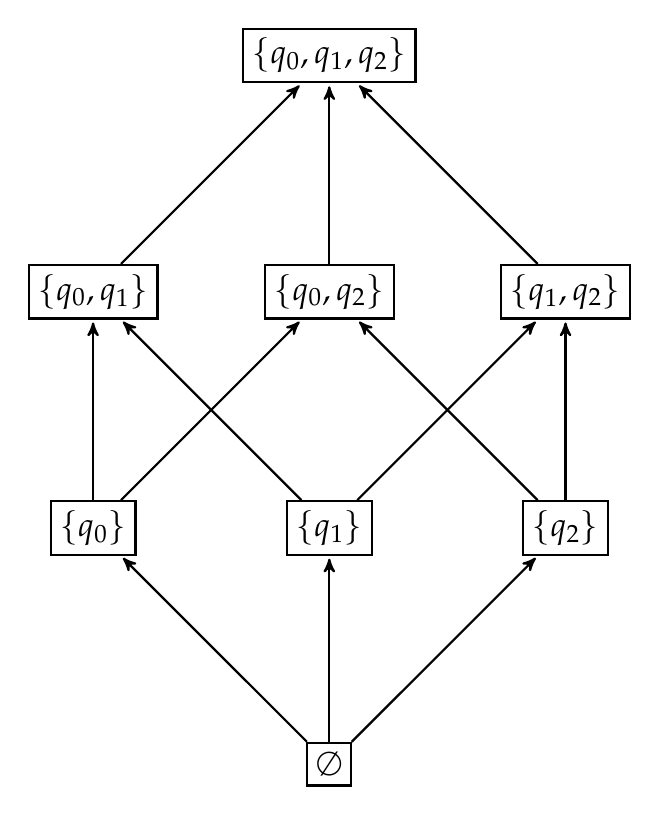
\begin{tikzpicture}[->,>=stealth',shorten >=1pt,auto,node distance=3cm,
                        thick,
                        main node/.style=
                        {rectangle,draw,font=\sffamily\large\bfseries}]

      \node[main node] (012) {$\{q_0, q_1, q_2\}$};
      \node[main node] (02) [below of=012] {$\{q_0, q_2\}$};
      \node[main node] (01) [left of=02] {$\{q_0, q_1\}$};
      \node[main node] (12) [right of=02] {$\{q_1, q_2\}$};
      \node[main node] (1) [below of=02] {$\{q_1\}$};
      \node[main node] (0) [left of=1] {$\{q_0\}$};
      \node[main node] (2) [right of=1] {$\{q_2\}$};
      \node[main node] (EMPTY) [below of=1] {$\emptyset$};

      \path[every node/.style={font=\sffamily\small}]
          (02) edge node [] {} (012)
          (01) edge node [] {} (012)
          (12) edge node [] {} (012)

          (0) edge node [] {} (01)
              edge node [] {} (02)
          (1) edge node [] {} (01)
              edge node [] {} (12)
          (2) edge node [] {} (02)
              edge node [] {} (12)

          (EMPTY) edge node [] {} (0)
                  edge node [] {} (1)
                  edge node [] {} (2)
        ;
    \end{tikzpicture}
    \caption{Example of antichains using
    the poset $\tuple{2^{Q_A}, \subseteq}$,
    With $Q_A$ the set of state of the automaton $A$, which correspond
    to $Q_A = \{q_0, q_1, q_2\}$. Each directed edge of the graph
    correspond to a valid comparison using the set inclusion $\subseteq$.
    For example
    $\{q_0\} \rightarrow \{q_0, q_1\}$ corresponds to
     the inclusion $\{q_0\} \subseteq \{q_0, q_1\}$. Two elements of the graph
     with no connection, means that the elements are incomparable. For
     example, $\alpha = \{\{q_0\}, \{q_1\}, \{q_2\}\}$ is a set
     of incomparable elements and $\alpha$ is called an antichain.}
     \label{fig:eg_antichain1}
\end{figure}

\todo{Fix figure formulation as we havent spoke about antichains at this
section yet}

\end{example}

\paragraph{Lattices} A \textit{lower semilattice} is a poset
$\tuple{S, \preceq}$ where for all pair of elements $s_1, s_2 \in S$,
we have that the greatest lower bound $s_1 \sqcap s_2$ exists.

\subsection{Antichains}

\subsubsection{Closed sets}

\paragraph{}


A closed set is a set $L \subseteq S$
of a lower semilattice $\langle S, \preceq \rangle$
where $\forall \ell \in L$ we have that $\forall s \in S$ such that
$s \preceq \ell$, then $s \in L$.

Note that for two closed sets $L_1, L_2 \subseteq S$, we have that
$L_1 \cup L_2$ and $L_1 \cap L_2$ are also closed sets,
but $L_1 \setminus L_2$ does not result necessarily to a closed set.

\paragraph{Maximal/minimal elements} We denote by $\ceil{L}$
the set of maximal elements of a closed set $L$ which
\todo{Meaning of | vs . vs : in set definition ?}
correspond to $\ceil{L} =
\{ \ell \in L | \forall \ell' \in L : \ell \preceq \ell'
 \Rightarrow \ell = \ell' \}$. Alternatively, to represent the set of minimal
 elements, the noation $\floor{L}$ is used which has the following semantic
$\floor{L} = \{ \ell \in L | \forall \ell' \in L :  \ell' \preceq \ell
 \Rightarrow \ell = \ell' \}$.


\paragraph{Closure} A \textit{lower closure} of a set $L$ on $S$
noted $\darrow L$ is the set of all elements of $S$ that are
\textit{smaller or equal} to an element of $L$ i.e.
$\darrow L = \{ s \in S \ | \ \exists \ell \in L \cdot s \preceq \ell\}$.
Note that for a closed set $L$ we have that $\darrow L = L$.



\paragraph{Antichain}

An antichain of a poset $\tuple{S, \preceq}$
is a set $\alpha \subseteq S$ where all element of $\alpha$
are incomparable with respect to the partial order $\preceq$.
Antichains allow to represent closed set in a more compact way.
For a closed set $L \subseteq S$ we can retrieve all elements of $L$ by using
the antichain $\alpha = \ceil{L}$. With respect
to the definition of the lower closure we have that $\darrow \alpha = L$.

\subsection{Operations on antichains}

\todo{Cite original paper, FJR11 from Bohy' phd}



\begin{proposition}

\label{antichains_ops}

Let $\alpha_1, \alpha_2 \subseteq S$ two antichains and $s \in S$:

\begin{itemize}
    \item $s \in \darrow \alpha_1$
    iff $\exists a \in \alpha_1$ such that $\preceq a$
    \item $\darrow \alpha_1 \subseteq \darrow \alpha_2$
    iff $\forall a_1 \in \alpha_1,
    \exists a_2 \in \alpha_2$ such that $a_1 \preceq a_2$
    \item $ \darrow \alpha_1 \ \cup \darrow \alpha_2 =
    \darrow \ceil{\alpha_1 \cup \alpha_2}$
    \item $\darrow \alpha_1 \ \cap \darrow \alpha_2 =
    \darrow \ceil{\alpha_1 \sqcap \alpha_2}$

\todo{Give complete definition for interesection}

\end{itemize}

\end{proposition}



% \subsection{Pseudo-antichains}
%
% \paragraph{}
%
% An antichain is a subset of $S$ that allow to represent in a compact way
% a set $L \subseteq S$ that is not necessarily closed.

\newpage

\section{Implementation}

\paragraph{}

Java already provide built-in implementation for \texttt{Set}.
\todo{Includes limitation of Java built-in and different possible solution
for antichains found on stack overflow and others}

\paragraph{}

In this thesis we are more interested in partially ordered sets as
totally ordered sets are already implemented
in\texttt{Java} built-in
\texttt{SortedSet}.

\subsection{Summary of objectives}


\paragraph{}


The main focus of the thesis is to be able to provide an efficient
implementation of antichains and pseudo-antichains in \texttt{Java}.
The first step is to provide an interface for the different operations that
can be applied to antichains. We then give a description
of the implementation.
Antichains provide a way to represent
in a compact way partially ordered set that are closed. Pseudo-antichains
are an extension of antichains and provide a compact way to represent
partially ordered sets. Pseudo-antichains does not specifically require
closed set.

Our goal is to find a way to not keep all the closure all
element of the antichain in memory, but be able to retrieve those elements
or check the belonging of a closure element from the incomparable elements
of the antichain.

\subsection{Existing implementation}

\todo{Discuss impl. specifics etc in chapter Implementation}
\todo{What operations are implemented in those papers ?}
\todo{What domain (of sets) is is used in those papers ?}
\todo{Research other possible related works}
\todo{ABout impl, should i talk about BDD ?}

\subsubsection{AaPAL}

\todo{Talk about AaPAL in Acacia+ ?}

Bohy's \textbf{A}ntichain
\textbf{a}nd \textbf{P}seudo-\textbf{A}ntichain \textbf{L}ibrary \cite{aapal}
is an open-source generic library for the manipulation
of antichains and pseudo-antichains data structures,
implemented in \texttt{C}. In this section we will mainly focus
on the implementation of antichains.
\todo{Pseudo-antichains might be interesting for next year maybe ?}


\paragraph{Antichain representation}

An antichain is represented by a \texttt{struct}, containing as attributes
the size of the antichain, and the incomparable elements of the antichains,
as a list. The list is manipulated using the \texttt{GSList} object
from the \texttt{glib} library.
\todo{Cite glib library}
To allow modularity, the type of the elements
is \texttt{void}.
\todo{Find usage of AaPAL (see Bohy's PHD)}

\paragraph{Operations}

The operations implemented in \texttt{AaPAL}
are the union, intersection and appartenance
defined in Proposition \ref{antichains_ops}.
An interesting remark is that most of the complexity is given as a paramater
to the functions. For example the function to compare two elements in
an antichain is given as a parameter. It means that the complexity to define
the domain of the antichain, must be implemented in the compare function.
Same pattern goes for the intersection operation,
the function to compute the intersection must be provided by the user.
Also basic
operations such as creating an antichain,
adding an element to
an antichain, checking emptiness or cloning an antichain are implemented.
in \texttt{AaPAL}.

\subsubsection{Antichains for Dedekind numbers algorithms}

De Causemaecker and De Wannemacker only provide the executable of
their algorithm in their paper for
the Dedekind algorithm \cite{causemaecker1}. Hoedt proposed in \cite{hoedt}
a algorithm to find the ninth Dedekind number, which requires an representation
of antichains. The representation used is an extension of the implementation
proposed by De Causmaecker and De Wannemacker. The source of his
implementation was found in is personal GitHub \cite{hoedt_src}.
We will therefore only focus on the implementation
of Hoedt, which is an extension of the implementation proposed
by De Causmaecker and De Wannemacker, but by representing an antichains
using bitarray-like methods.

\paragraph{Antichains representation}

According to Hoedt in
\cite{hoedt}, the first proposed representation
in \cite{causemaecker1} was done by using
a \texttt{TreeSet}. With the objective to improve the performance of
the important operations, for example the intersection, Hoedt used
another way to represent antichains, by using a bitarray-like representation.
This representation

\subsection{Difficulties}

\todo{What is the difference beetween domain, univers and set ?}

One of the difficulties is to define the domain of the elements that
the antichains should work on. In \texttt{AaPAL} the all complexity
is implemented in the \texttt{compare\_elements} that must be given
to the library functions. It that case, all the complexity of the
must be implemented by the user to define the domain of the antichains.

\subsubsection{Tree vs Bitarray representations}


\subsection{Possible solutions}

In the case of the domain specifications, a good approach could be to
provide an interface/abstract class to the users, to let them provide
their own implementation. In addition to that, usual domain such a
natural numbers or others well known domain used, could be directly
implemented
in the library.


\subsection{New implementation}


\section{Next year overview}

\label{conclusion}

\subsection{Requirements}

Java + Owl

\todo{Talk about Owl}

The requirements of the

\subsection{Framework and implementation}

\paragraph{}

The interface proposed in \ref{oset_git} gives a first overview
of the desired implementation. The goal will be to try to find a good
way to implement antichains. One of the possible way to do so is to provide
operations depending on the universe of the antichains. For example,
the implementation of Hoedt presented in section \ref{sota_hoedts}
using bitarray can only be applied to natural numbers. An first step
is to proposed an framework for users to implement the specifics of the
universe necessary for their algorithms. The goal of the thesis will
be to propose a generic and abstract API, and implement specifics
for known universe and test them of state-of-the-art algorithms,
especially in automata theory.


\subsection{Possible extensions}


As we mainly focus on efficiency, it could be interesting to use a \texttt{C}
implementation such as \texttt{AaPAL},
and provide bindings to \texttt{Java}. We could try
this method as an alternative to a pure \texttt{Java} implementation and
compare performances.


\todo{Fill-in bib correctly!}

\bibliographystyle{alpha}
\bibliography{thesis}

\end{document}
